\documentclass[sigplan]{acmart}
\usepackage{subcaption}
\usepackage{caption}
\usepackage{array}
\usepackage{multirow}
%%
%% \BibTeX command to typeset BibTeX logo in the docs
\AtBeginDocument{%
  \providecommand\BibTeX{{%
    \normalfont B\kern-0.5em{\scshape i\kern-0.25em b}\kern-0.8em\TeX}}}

\setcopyright{none}
\copyrightyear{}
\acmYear{}
\acmDOI{}

\acmConference[]{Introduction to Research}{December 2021}{Lisbon}
\acmBooktitle{}
\acmPrice{}
\acmISBN{}


%% end of the preamble, start of the body of the document source.
\begin{document}

%%
%% The "title" command has an optional parameter,
%% allowing the author to define a "short title" to be used in page headers.
\title{Desenvolvimento de uma Aplicação em Orientação a Objetos}

%%
%% The "author" command and its associated commands are used to define
%% the authors and their affiliations.
%% Of note is the shared affiliation of the first two authors, and the
%% "authornote" and "authornotemark" commands
%% used to denote shared contribution to the research.

\author{Pedro Miguel Ferreira Tavares Carrega - 49480}
\affiliation{
 \institution{ Estudo Orientado em Engenharia Informática \\ Mestrado em Engenharia Informática \\ Faculdade de Ciências, Universidade de Lisboa}
 }
\email{fc49480@alunos.fc.ul.pt}


\renewcommand{\shortauthors}{Pedro Miguel Ferreira Tavares Carrega - 49480}

%%
%% The abstract is a short summary of the work to be presented in the
%% article.
\begin{abstract}
Este relatório foi desenvolvido com o propósito de descrever o ambito do tema de tese a ser entregue no fim do atual ano lectivo e detalhar o trabalho até agora realizado no trabalho de projeto. A minha tese encontra-se a ser realizada na empresa ARTSOFT, uma empresa com dezenas de anos de experiência a desenvolver soluções de gestão empresarial, em particular o desenvolvimento e comercialização da aplicação ERP ARTSOFT. O propósito da minha tese vai ser a integração dos \textit{web services} fornecidos pela Segurança Social e pelos Fundos de Compensação na aplicação ERP ARTSOFT, sendo que este relatório vai relatar todo o trabalho até agora realizado no ambito da minha tese.
\end{abstract}


%%
%% Keywords. The author(s) should pick words that accurately describe
%% the work being presented. Separate the keywords with commas.
\keywords{ERP ARTSOFT, OOP, C++, Segurança Social, Fundos de Compensação}


%%
%% This command processes the author and affiliation and title
%% information and builds the first part of the formatted document.
\maketitle

\section{Introduction}

\textit{Enterprise Resource Planning} ARTSOFT é uma aplicação de gestão empresarial que é estruturada em vários modulos, oferecendo ao utilizador uma aplicação que se adapte as suas necessidades. Atualmente um utilizador da aplicação ERP ARTSOFT que queira submeter o vínculo do seu novo trabalhador tem de utilizar a plataforma online disponibilizada pela Segurança Social; este processo não é eficiente. O atual processo obriga o utilizar a submeter duas vezes a mesma informação, primeiro terá de criar a entrada do seu novo empregado na base de dados da aplicação ERP ARTSOFT, tendo de seguida submeter os dados do trabalhador na plataforma da Segurança Social. Num contexto empresarial este gasto adicional de tempo é muito caro para uma empresa, então foi inicializado um desenvolvimento com o objetivo de oferecer ao cliente a possibilidade de submeter o vínculo de contrato do seu novo trabalhador à Segurança Social diretamente da aplicação ERP ARTSOFT. Outra funcionalidade oferecida pelo \textit{web service} da Segurança Social é a submissão e atualização da declaração mensal de rendimentos. Esta funcionalidade resolve o mesmo problema que a entrega do vínculo de trabalhador resolve a perda desnecessária de tempo, atualmente o utilizador pode gerar esta declaração diretamente da aplicação ERP ARTSOFT contudo para submeter ou atualizar terá de utilizar a plataforma online da Segurança Social. O \textit{web service} dos Fundos de Compensação oferece três diferentes serviços, sendo os três relacionados com o estado de trabalhadores numa empresa permitindo reportar a admissão de um novo trabalhador, o terminar de contrato de um trabalhador e a atualização dos dados de um contrato sendo que estas três funcionalidades tem o mesmo objetivo, tal como o \textit{web service} da Segurança Social, poupar tempo ao utilizador. Com o propósito de integrar os \textit{web services} apresentados será inicializado um processo de desenvolvimento, começando pela redação de uma especificação de requisitos cuja análise permite a formalização do desenvolvimento a ser efetuado, baseada no estudo da aplicação ERP ARTSOFT e a documentação dos \textit{web services} a integrar; após a aprovação da especificação e utilizando uma metologia agile, serão realizados SPRINTS quinzenais concluindo com uma bateria testes funcionais aos serviços integrados. Para iniciar este relatório vai ser primeiro introduzido e explicado alguns conceitos base para entender como funcionam os modulos relevantes da aplicação ERP ARTSOFT e alguns dos procedimentos internos na empresa. De seguida vai ser apresentado um relato da formação realizada, seguida de uma análise da documentação dos \textit{web services} a implementar, uma apresentação dos metodos que foram e irão ser utilizados para resolver o problema apresentado e por fim serão apresentados os próximos passos a realizar para chegar à solução do problema.

\section{Background} \label{sec:background}

\subsection{Ferramentas Utilizadas}

\subsubsection{ERP ARTSOFT}

ERP ARTSOFT é o nome da aplicação desenvolvida na empresa ARTSOFT e é crucial para todo o desenvolvimento efetuado na empresa. Internamente são utilizadas várias funcionalidades da aplicação, em particular, workflows e a criação e gestão de eventos. 

\subsubsection{TortoiseSVN}

O TortoiseSVN é um cliente \textit{open source} para a aplicação Apache Subversion oferecendo uma interface gráfica, um submenu de contexto no explorador do windows e acesso rápido a todos os comandos oferecidos pelo Subversion. Subversion é uma aplicação de controlo de versões que corre num servidor centralizado. Uma arquitetura centralizada oferece várias vantagens em comparação com uma arquitetura distribuída: O repositório encontra-se hospedado num servidor central, retirando a necessidade de clonar o repositório na sua totalidade. Isto também permite a atualização somente dos ficheiros locais. Ambos estes fatores levam a uma carga inferior da rede, contudo também implica se o servidor central se encontrar em baixo também se encontra o serviço. Subversion também permite a definição de restrição de acessos e o bloqueio de escrita simultânea de ficheiros, impedido o merge de binários.

\subsubsection{Jenkins}

\textit{DevOps} é um conjunto de filosofias e práticas que promovem o desenvolvimento e lançamento de aplicações com maior rapidez e qualidade. Duas das práticas mais relevantes são \textit{Continuous Integration} e \textit{Continuous Delivery}. \textit{Continuous Integration} é uma prática aonde programadores integram, com regularidade, código desenvolvido para um repositório central sendo automaticamente compilado e efetuados testes sobre o mesmo. Este depois é automaticamente preparado para lançamento, sendo esta a base de \textit{Continuous Delivery}. Com o objetivo de promover estas práticas a empresa ARTSOFT usa a ferramenta Jenkins - um servidor de automação \textit{open source} que corre em \textit{servlet containers} facilitando \textit{Continuous Integration} e \textit{Continuous Delivery} através de \textit{pipelines} para automizar a compilação de binários através da definição de um conjunto de processos que permitem às pipelines compilar, construir e lançar automaticamente o código produzido.

%adicionar imagem de 1 pipeline

\subsection{Eventos}

Um evento é um registo interno que é criado na aplicação ERP ARTSOFT sempre que ocorra um acontecimento. Dentro da empresa ARTSOFT é utilizado para efetuar o registo de vários tipos de acontecimentos sendo os mais comuns os eventos de reporte de bugs e eventos de roadmap. Roadmap são eventos que envolvem o desenvolvimento de funcionalidades para futuras versões do ARTSOFT. Eventos que reportam bugs no funcionamento da aplicação ARTSOFT, estes eventos podem ser criados devido a reportes internos ou por clientes da aplicação ARTSOFT. Na criação de um evento o utilizador tem obrigatoriamente de fornecer as seguintes informações: o cliente do evento, o tipo de evento e o assunto do evento; adicionalmente é possível adicionar uma mensagem para descrever o evento em mais detalhe e até adicionar imagens. No contexto de um reporte de bug ou roadmap é necessário indicar a que modulo do ERP ARTSOFT este evento se enquadra, esta informação toda é possível ser visualizada na imagem abaixo.

\begin{figure}[htbp]
	\centerline{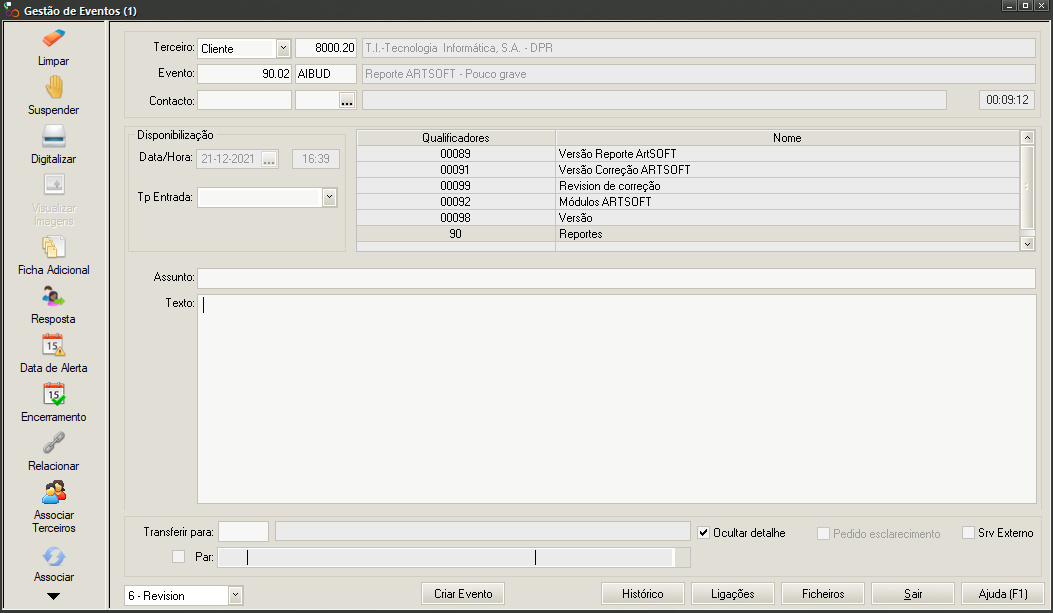
\includegraphics[width=\linewidth]{figures/evento_criacao.png}}
	\caption{Criação de um evento}
	\label{fig1}
\end{figure}

Um evento de bug ao ser criado é enviado para a entrada do Departamento de Programação (DRP), aí o mesmo é atribuído a um membro da equipa. O programador responsável pelo evento ao concluir o seu trabalho transfere o evento para a Unidade de Qualidade de Software (UQS). A equipa de testes vai testar o evento, confirmando se o mesmo se encontra resolvido. Caso o evento se encontre resolvido é assinalado como tal e é passado para a saída do DPR, senão o evento é passado de volta para o programador responsável pelo evento.

\subsection{Formação}

Os primeiros três meses da minha tese foram dedicados à minha formação. O primeiro dia foi dedicado a ensinar-me os conceitos básicos do funcionamento da aplicação ARTSOFT, o funcionamento das ferramentas utilizadas para o controlo de versões e como funciona o fluxo de um evento. O restante da minha primeira semana foi dispendido a tratar de um evento de tipo roadmap, evento que foi criado somente com o propósito de formação, que me deu contacto com tudo que iria necessitar para efetuar desenvolvimento na aplicação ARTSOFT. O evento pedia a criação de uma interface que, dado um de três tipos de entradas: Diário, Documento, Conta, apresentasse ao utilizador transações presentes na entrada selecionada. Os três tipos de entradas requerem o número da entrada a consultar, sendo possível fornecer diferentes tipos consoante o tipo de entrada para filtrar os resultados. O diário é possível limitar ao mês que se pretende consultar enquanto que o documento é possível filtrar por tipo de documento. Na seguinte imagem é possível visualizar o evento acima descrito e as algumas das mensagens registadas durante o desenvolvimento da funcionalidade descrita.

\begin{figure}[htbp]
	\centerline{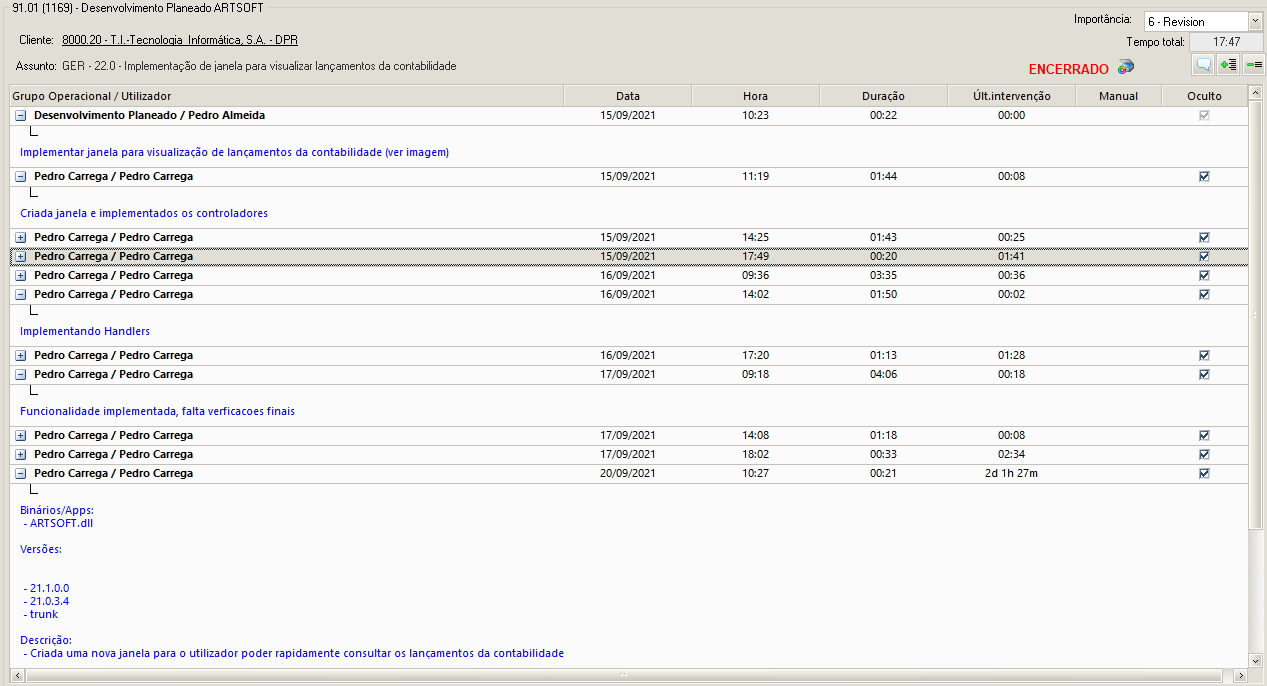
\includegraphics[width=\linewidth]{figures/evento_formacao.png}}
	\caption{Registo do evento de formação}
	\label{fig2}
\end{figure}

\subsubsection{Diário}

\subsubsection{Documento}

\subsubsection{Conta}

\subsubsection{Conhecimentos Adquiridos}

%Este desenvolvimento é perfeito para introduzir um programador a trabalhar com a linguagem C++ e a utilizar as ferramentes já existentes na aplicação ARTSOFT. Ao ter de criar uma interface gráfica 
 Após a entrega desta nova funcionalidade foi me atribuído regularmente diferentes eventos até o prazo que se inicializou o desenvolvimento na nova versão do ARTSOFT.

\section{Data} \label{sec:data}

%Falar da documentação dos web services
Here you should describe your data in as much detail as possible. \\ 

You can describe raw data and any pre-processing need for your work. \\

You can have a section on exploratory data analysis. \\

\section{Methods} \label{sec:methods}

Here you should describe in as much details as possible the problem and your plan to tackle it. \\

What are the methods you are planning to use, or already started to use, to tackle your problem. \\

This should be based on related word, your understanding of the problem and eventually preliminary exploratory data analysis or preliminary results.

\subsection{Problema} %alterar o nome desta seccao

\subsection{Redação da Especificação de Requisitos}

\subsection{Sprints}

\subsection{Testes}

\section{Forthcoming Work} \label{sec:forthcomingwork}

%Here you should write the conclusion of the preliminary work and the goals for the remaining period.

O passo seguinte a realizar no projeto será a realização de uma reunião para apresentar e aprovar a especificação de requisitos. Dada a aprovação, utilizando uma metodologia agile, serão definidos vários SPRINTS quinzenais com diferentes objetivos vão ser implementadas as interfaces gráficas e requisitos descritos na especificação. Uma vez implementadas, irá ser utilizado o ambiente de qualidade para realizar testes de forma a confirmar o correto comportamento das funcionalidades implementadas. Estas novas funcionalidades irão ser incluídas na nova versão da aplicação ARTSOFT, aonde será realizado tratamento de bugs que surgam nas funcionalidades implementadas.

%%
%% The next two lines define the bibliography style to be used, and
%% the bibliography file.
\bibliographystyle{ACM-Reference-Format}
\bibliography{bib/bibliography}
\end{document}

\endinput
%%
%% End of file.
